%----------- File: Kapitel/gui.tex -----------

\chapter{Überblick über die Applikation}
\label{chap:ueberblick}
\authormargin{Mike Wild}

In diesem Kapitel wird die entwickelte Applikation vorgestellt. Ziel ist es, einen umfassenden Eindruck von den vorhandenen Funktionalitäten sowie der grafischen Benutzeroberfläche zu vermitteln. Dabei werden zunächst die zentralen Anwendungsbereiche und Hauptfunktionen erläutert. Anschließend erfolgt eine Darstellung der Benutzeroberfläche, um den Aufbau und die Bedienlogik der Software nachvollziehbar zu machen. Auf diese Weise wird ein zusammenhängendes Bild des Systems geschaffen, das sowohl die technischen Kernkomponenten als auch die praktische Nutzung aus Anwendersicht verdeutlicht.

\section{Zielsetzung und Einsatzbereich}
\label{sec:ziel}
\authormargin{Mike Wild}

Diese Applikation wurde entwickelt, um Online-Meetings zu protokollieren. Dabei ist es egal, mit welchem Programm das Meeting geführt wird oder auf welchem Betriebssystem, ob Windows, Linux oder MacOS. Ziel ist es die automatische Transkription in Echtzeit durchzuführen und die Transkripte in einer Datenbank zu speichern und zu verwalten. Das Programm bietet jedoch Potential, um auch in anderen Anwendungsbereichen eingesetzt zu werden (siehe dazu Kapitel \ref{chap:fazit_ausblick}, Seite \pageref{chap:fazit_ausblick}). Die nachfolgend eingefügten Bilder der Benutzeroberfläche zeigen das Aussehen auf ein Linux-System mit systemseitig dunklen-Theme eingestellt.


\section{Funktionsumfang}
\label{sec:umfang}
\authormargin{Mike Wild}

Um ein Meeting vollständig erfassen zu können, benötigt man neben dem Audiosignal des Mikrofons, was nur die eigene Stimme aufzeichnet, auch die Stimmen der anderen Teilnehmer. Deshalb greift die Applikation auch auf den Systemmix, das Ausgangs-Audiosignal, das an die Lautsprecher bzw. Kopfhörer geht, zu. Mikrofon-Audio und Systemmix werden gemischt und aufgezeichnet. Diese Aufzeichnung kann hinterher als Audiodatei gespeichert werden, um sich das Meeting oder Teile davon erneut anzuhören. Das erfasste Audiosignal wird entweder in Echtzeit oder nachgelagert von einem lokal-laufenden \ac{KI}-Modell transkribiert, wobei auch nach Sprecher getrennt wird. Mithilfe der Applikation ist es möglich das Transkript zu manipulieren, um Fehler der Transkription zu korrigieren oder den, von der \ac{KI} erkannten Sprecher, echte Namen zuzuordnen. Das Transkript kann sowohl in der Datenbank, als auch als JSON-Datei gespeichert werden (siehe Abbildung \ref{pic:json}). Des Weiteren ist ein Export als PDF-Datei möglich (vgl. Abbildung \ref{pic:pdf}). Der Transkription können auch noch Schlagworte, sogenannte Tags, automatisch hinzugefügt werden.


\begin{figure}
    \centering
    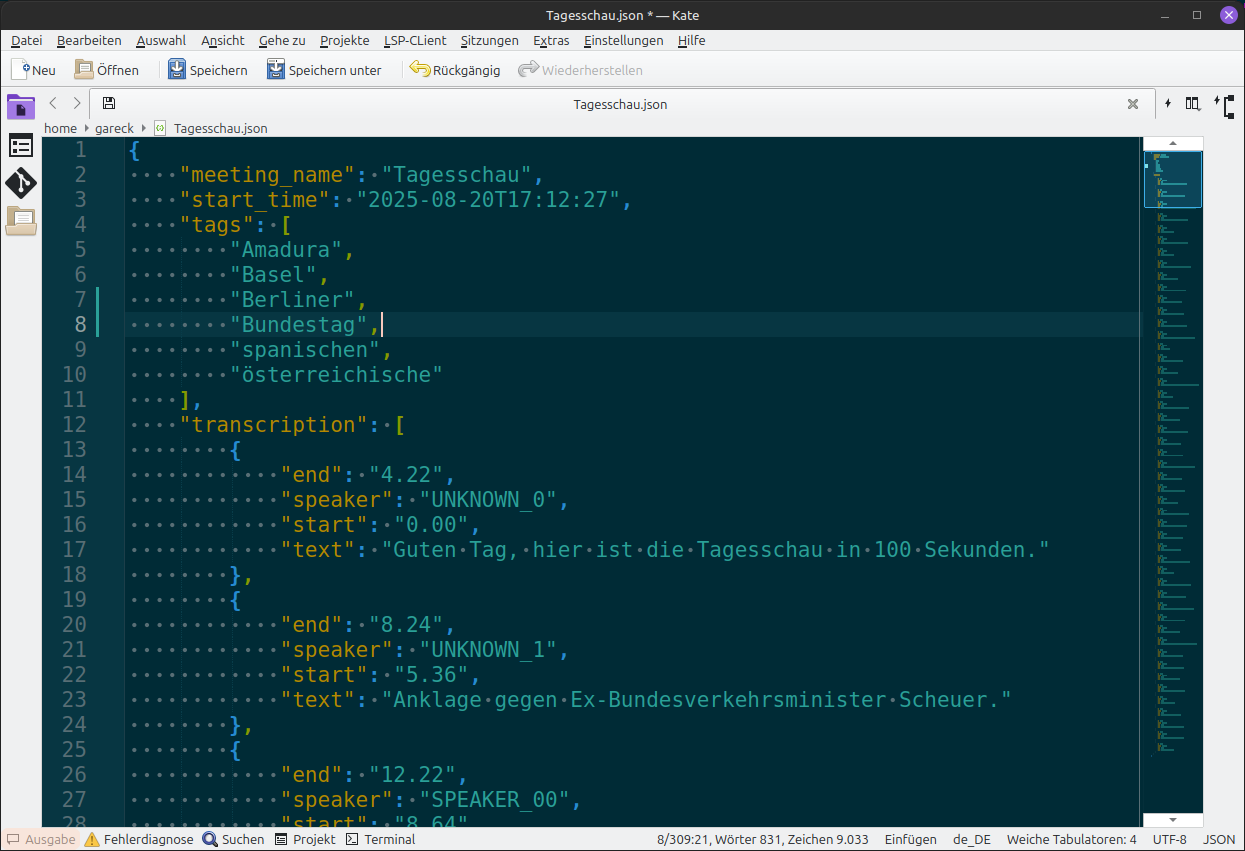
\includegraphics[width=0.7\linewidth]{Bilder/JSON}
    \caption[JSON]{Ausschnitt einer exportierten JSON-Datei in einem Texteditor}
    \label{pic:json}
\end{figure}


\begin{figure}
    \centering
    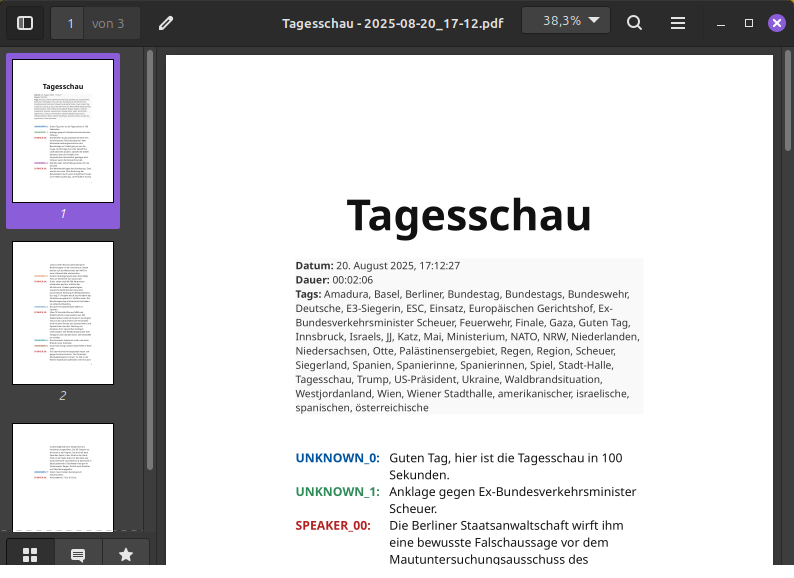
\includegraphics[width=0.7\linewidth]{Bilder/PDF}
    \caption[PDF]{Anfang eines Transkriptes im PDF-Format}
    \label{pic:pdf}
\end{figure}





\section{Anleitung und Benutzeroberfläche}
\label{sec:gui}
\authormargin{Mike Wild}

\subsection{Python-Installationsfenster}
\label{sub:install}

Wenn man das Programm das erste Mal startet, öffnet sich nicht das Hauptfenster der Anwendung, sondern es wird automatisch eine virtuelle Python-Umgebung eingerichtet, die alle benötigten Pakete und \ac{KI}-Modelle für die Transkription und andere Funktionen beinhaltet. Dies dient dazu, dass das Programm das System, auf dem es läuft, nicht verändert. Abbildung \ref{pic:Install} zeigt das Installationsfenster für die virtuelle Python-Umgebung. Die Installation übernimmt ein Shell- bzw. Batch-Skript. Die Ausgabe des Skripts wird im Fenster angezeigt. Das Skript kann später über den Menü-Punkt "Python neu-installieren" oder auch manuell erneut gestartet werden. Die nun installierte virtuelle Umgebung ist nicht zwangsläufig notwendig. Man kann die Installation abbrechen und das auf dem System installierte Python nutzen. Hierzu wird nach dem Abbrechen oder bei einem Installationsfehler zunächst das Einstellungsfenster (siehe Abb. \ref{pic:Settings} geöffnet.

\begin{figure}
    \centering
    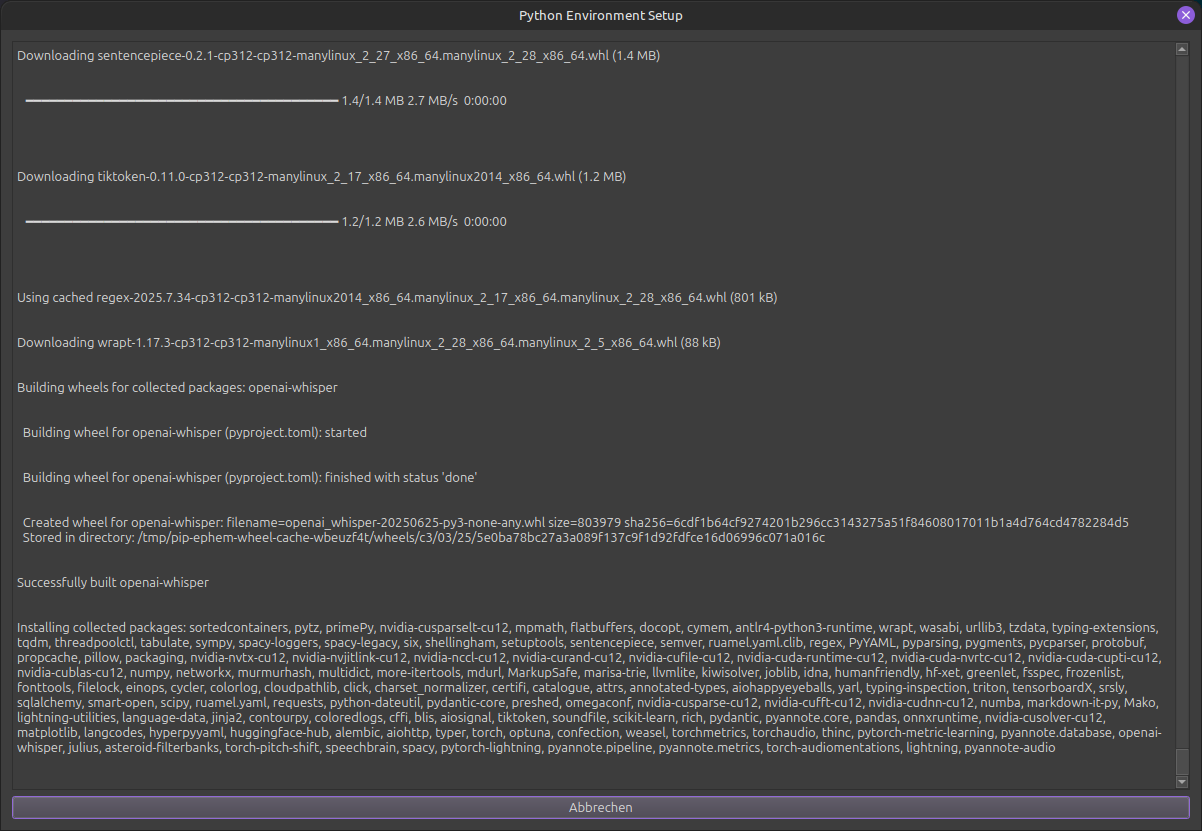
\includegraphics[width=0.7\linewidth]{Bilder/Python-Installationsfenster}
    \caption[Python-Installationsfenster]{Python-Installationsfenster}
    \label{pic:Install}
\end{figure}


\subsection{Einstellungsfenster}
\authormargin{Mike Wild}

\begin{figure}
    \centering
    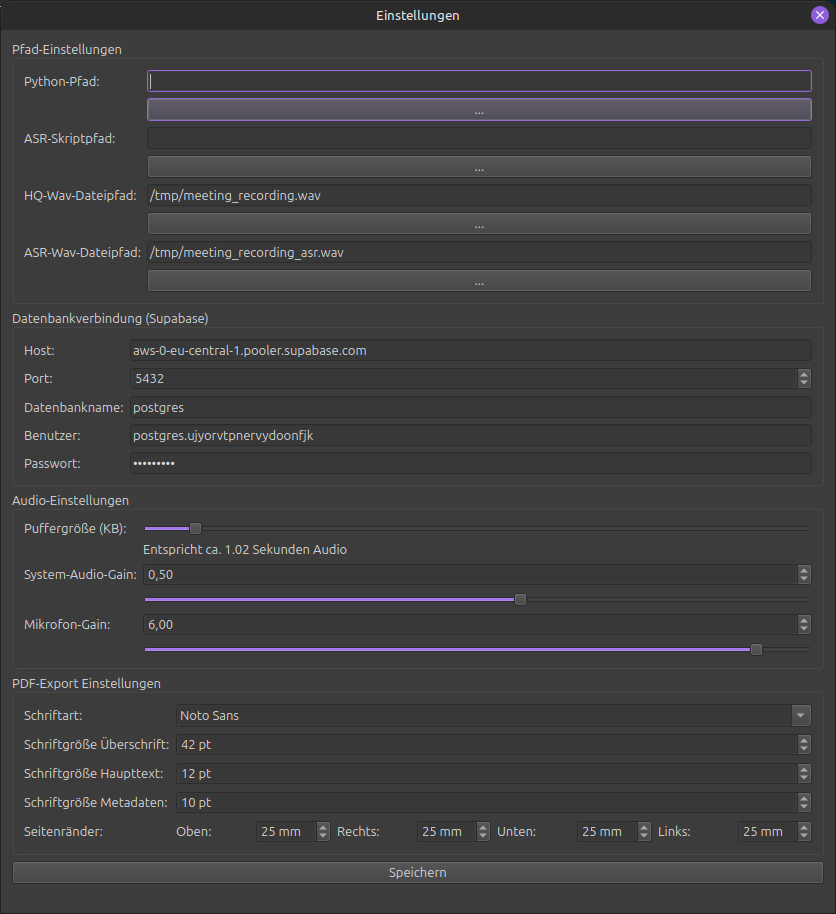
\includegraphics[width=0.7\linewidth]{Bilder/Einstellungen}
    \caption[Einstellungsfenster]{Einstellungsfenster}
    \label{pic:Settings}
\end{figure}


Dort muss unter dem Punkt \glqq Python-Pfad\grqq\ der Pfad zur ausführbaren Python-Datei (meist \glqq python3\grqq\ genannt) eingetragen werden. Hier kann die Datei aus einer beliebigen virtuellen Umgebung oder die Datei vom System eingetragen werden. Unter dem zweiten Punkt \glqq ASR-Skriptpfad\grqq\ muss ein Python-Skript zum Transkribieren eingetragen werden. Das Programm bietet momentan die beiden Möglichkeiten \glqq run\_asr.py\grqq\ und \glqq asr\_backend.py\grqq. Das erste Skript transkribiert das Audio erst hinterher, indem es eine Wav-Datei entgegennimmt. Es arbeitet mit pyannote und whisper. Das zweite Skript ist für die Echtzeitverarbeitung zuständig, näheres im Kapitel \ref{chap:ki} auf Seite \pageref{chap:ki}. Diese ersten zwei Punkte sind essentiell, damit das Programm wie vorgesehen arbeiten kann.

Mit den nächsten zwei Pfaden kann man angeben, wo das Programm die Audiodateien zwischenspeichert. Diese werden im Wav-Format gespeichert. Dabei steht \glqq HQ\grqq\ für \textbf{H}igh-\textbf{Q}uality, also die Audiodatei mit voller Qualität, und \glqq ASR\grqq\ für die downgesamplete Audiodatei zur nachträglichen Transkription. Standardmäßig werden für die diese beiden Dateien in einem Standardordner für temporäre Dateien gespeichert. Danach folgen Einstellungen zur Datenbankverbindung, wo die Transkripte gespeichert und abgerufen werden sollen. Hier ist eine \glqq Supabase\grqq\ Datenbank vorgesehen, kann aber ggf. durch eine andere Datenbank ausgetauscht werden, die im Qt-Framework vom Typ \glqq QPSQL\grqq\ ist und mit denselben Parametern sich verbinden lässt. Anschließend folgend die Audio-Einstellungen. Die Puffergröße bestimmt wie viel Audio-Daten zwischengespeichert werden, bevor sie auf die Festplatte in die Wav-Dateien geschrieben werden. Die beiden Gain-Werte ergeben das Mischungsverhältnis zwischen Mikrofon- und Systemaudio-Lautstärke. Diese sollten so eingestellt werden, dass in der resultierenden Audio-Datei die Lautstärke des Mikrofons genauso laut ist, wie die des Systemmix. Zuletzt folgen noch Einstellungen, um das Aussehen der PDF-Datei, die man aus dem Transkript erzeugen lassen kann, zu optimieren.


\subsection{Hauptfenster}
\authormargin{Mike Wild}
\label{sub:main}

\begin{figure}
    \centering
    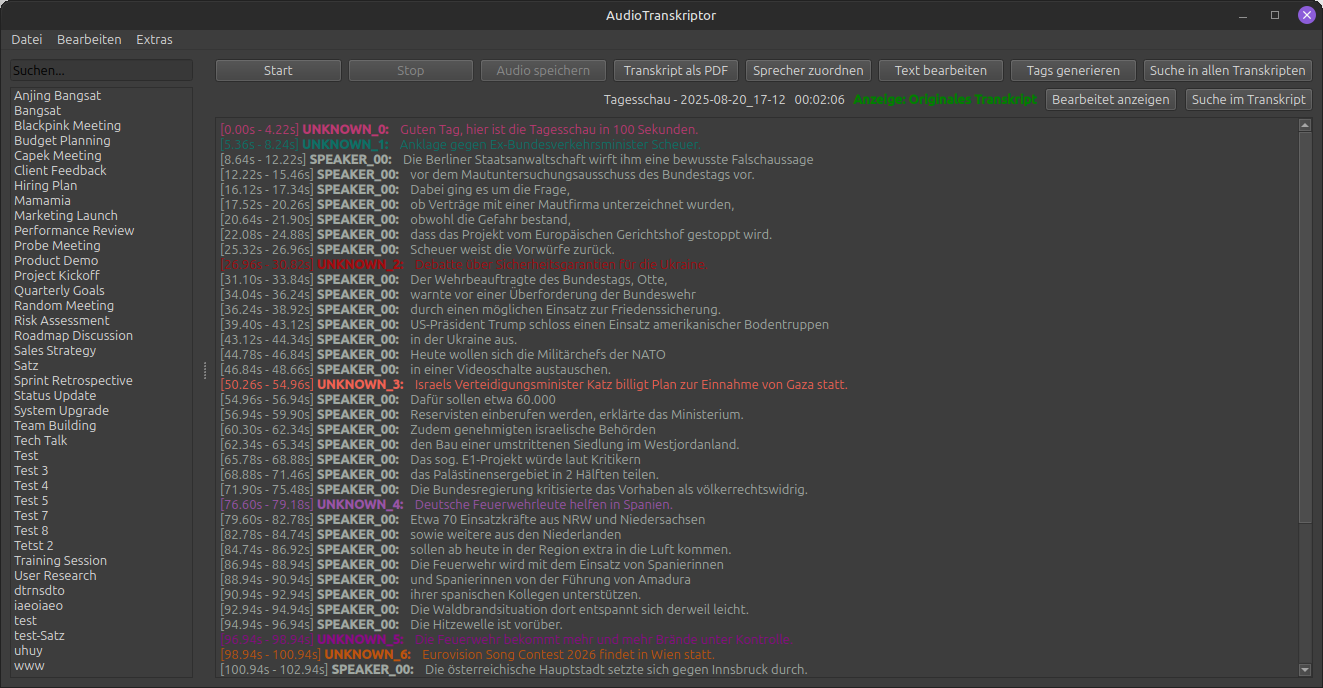
\includegraphics[width=0.7\linewidth]{Bilder/Applikation}
    \caption[Hauptfenster]{Hauptfenster der Applikation}
    \label{pic:App}
\end{figure}

Im Hauptfenster der Applikation befindet sich ganz oben die Menü-Leiste mit der man Transkripte speichern und laden kann, Änderungen rückgängig machen, Python neu installieren kann und das Einstellungsfenster öffnet. Bei MacOS befindet sich die Menüleiste nicht im Fenster, sondern am oberen Bildschirmrand. Auf der linken Seite sieht man die in der Datenbank gespeicherten Transkripte. Auf der rechten Seite sieht man zentral das gerade geladene Transkript und oberhalb davon die Bedienelemente. \glqq Start\grqq\  bzw. \glqq Stopp\grqq\  starten bzw. stoppen die Audioaufnahme. Erst nachdem eine Aufnahme beendet worden ist, kann man mit \glqq Audio speichern\grqq\ diese als Wav-Datei speichern. \glqq Transkript als PDF\grqq\  dient zum Exportieren des Transkriptes als PDF-Datei. \glqq Sprecher zuordnen\grqq\ (siehe Abschnitt \ref{sub:sprecher}) und \glqq Text bearbeiten\grqq\ (siehe Abschnitt \ref{sub:text}) dienen zum Manipulieren des Transkriptes. Mit \glqq Tags generieren\grqq\ werden über ein Python-Skript mittes spaCy Schlagworte zum gesamten Transkript erzeugt.

\authormargin{Yolanda Hadiana Fiska}
Der Button „Bearbeitet anzeigen“ ermöglicht es dem Benutzer, die Ansicht des geladenen Transkripts abhängig vom aktuellen Modus umzuschalten. Während die Option „Bearbeitet anzeigen“ zur redigierten Version des Transkripts wechselt, führt die Option „Original anzeigen“ zurück zur ursprünglichen Fassung. Der jeweils aktive Modus wird links neben diesem Umschaltknopf angezeigt. Darüber hinaus stehen dem Benutzer zwei Funktionen zur Protokollsuche zur Verfügung: Mit „Suche im Transkript“ kann innerhalb des aktuell geladenen Transkripts nach bestimmten Begriffen, Diskussionspunkten oder Informationen gesucht werden (siehe Abschnitt \ref{sub:lokalesuche}), während „Suche in allen Transkripten“ eine suchübergreifende Recherche über sämtliche vorhandenen Transkripte hinweg ermöglicht (siehe Abschnitt \ref{sub:globalesuche}).

\subsection{Sprecherbearbeitung}
\authormargin{Mike Wild}
\label{sub:sprecher}

\begin{figure}
    \centering
    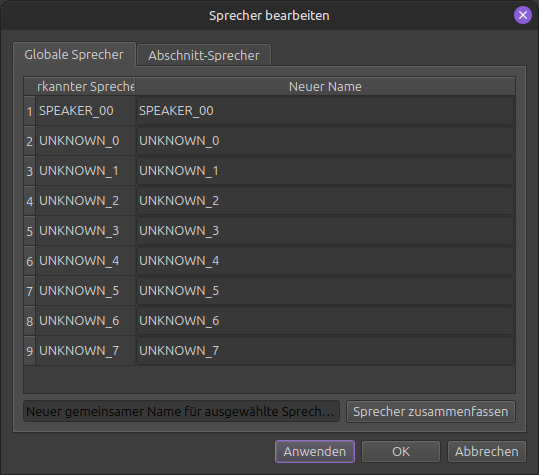
\includegraphics[width=0.7\linewidth]{Bilder/Sprecher1}
    \caption[Sprecherzuordnung]{Sprecherzuordnung für das gesamte Transkript}
    \label{pic:sprecher-allg}
\end{figure}

\begin{figure}
\centering
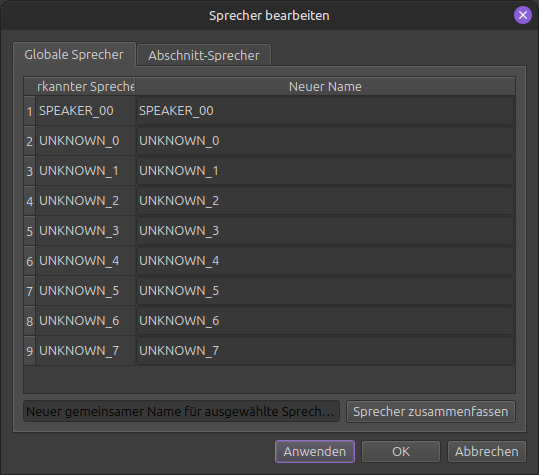
\includegraphics[width=0.7\linewidth]{Bilder/Sprecher1}
\caption[Sprecher ändern]{Sprecherzuordnung für einzelne Abschnitte}
\label{pic:sprecher-spez}
\end{figure}

Das Fenster zum Bearbeiten bzw. Zuordnen von Sprecher hat zwei Tabs, zwischen denen man wechseln kann. Der erste Tab (Abbildung \ref{pic:sprecher-allg}) dient dazu den Sprechern im Transkript, die automatisch mit \glqq SPEAKER\_XX\grqq\ (wobei XX eine zweistellige Nummer ist) benannt sind, echte Namen zuzuordnen. Das heißt, der Sprechername wird im gesamten Transkript ausgetauscht. Der zweite Tab (Abbildung \ref{pic:sprecher-spez}) ist dafür gedacht, falls die \ac{KI} den Text einen falschen Sprecher zuordnet, dies für diesen Textabschnitt zu korrigieren. Hier lassen sich die Spalten Start(-zeit) Ende (Endzeit) und Text nicht bearbeiten und dienen zum eindeutigen Erkennen des Abschnittes, von den man den Sprecher ändern möchte.


\subsection{Textbearbeitung}
\authormargin{Mike Wild}
\label{sub:text}

\begin{figure}
\centering
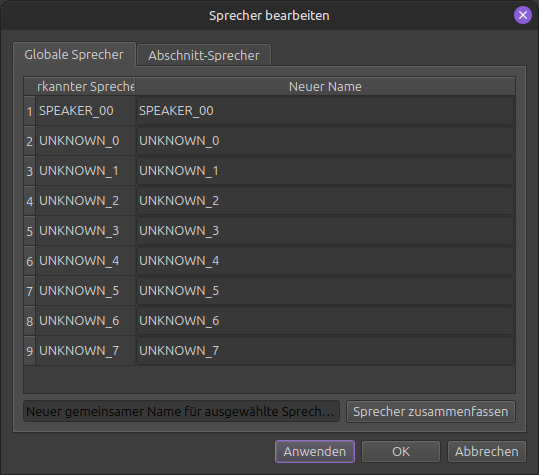
\includegraphics[width=0.7\linewidth]{Bilder/Sprecher1}
\caption[Textbearbeitung]{Textbearbeitung einzelner Abschnitte}
\label{pic:text}
\end{figure}

Mit dem Fenster in Abbildung \ref{pic:text} kann man den von der \ac{KI} automatisch transkribierten Text korrigieren, falls diese etwas fehlerhaft transkribiert hat. Die Spalten Start(-zeit) Ende (Endzeit) und Sprecher lassen sich hier nicht bearbeiten und dienen zum eindeutigen Erkennen des Abschnittes, den man bearbeiten möchte.

\subsection{Suche innerhalb eines Meetings}
\authormargin{Yolanda Hadiana Fiska}

\begin{figure}
\centering
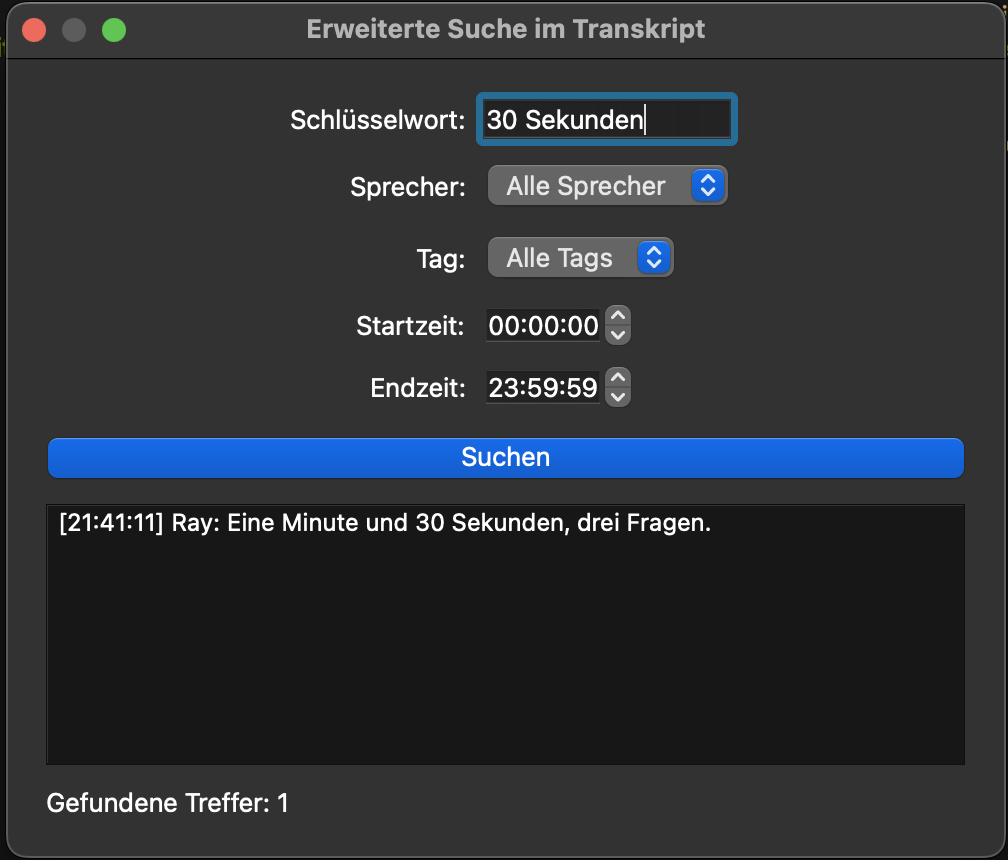
\includegraphics[width=0.7\linewidth]{Bilder/sucheInnerhalbMeeting.png}
\caption[Protokolsuche]{Systemansicht: Suche im Einzeltranskript}
\label{pic:lokalesuche}
\end{figure}

Das Fenster „Erweiterte Suche im Transkript“ (siehe Abbildung \ref{pic:lokalesuche} ) erlaubt eine gezielte Recherche innerhalb des aktuell geöffneten Transkripts. Es stellt verschiedene Such- und Filteroptionen zur Verfügung. Über das Feld „Schlüsselwort“ kann nach einem oder mehreren spezifischen Begriffen gesucht werden. Zusätzlich besteht die Möglichkeit, die Suche nach Sprecher (z. B. alle Sprecher oder ein bestimmter Redner) sowie nach Tags einzugrenzen. Ebenso können durch die Angabe einer Startzeit und Endzeit nur bestimmte Zeitbereiche des Transkripts berücksichtigt werden.

Die Ergebnisse der Suche werden in einer Liste dargestellt und enthalten die Zeitangabe, den Namen des Sprechers sowie die entsprechende Aussage. Wie in Abbildung \ref{pic:lokalesuche} dargestellt, werden die Eingabeoptionen für die Suche bereitgestellt.

\subsection{Globale Suche über alle Meetings}
\authormargin{Yolanda Hadiana Fiska}

Das Fenster „Erweiterte Mehrfachsuche“ (siehe Abbildung \ref{pic:globalesuche}) ermöglicht eine protokollübergreifende Recherche über sämtliche gespeicherten Transkripte. Im Unterschied zur Suche innerhalb eines einzelnen Protokolls werden hier alle verfügbaren Sitzungen in die Abfrage einbezogen. Die Filtermöglichkeiten entsprechen im Wesentlichen denen der Suche innerhalb eines Meetings, werden jedoch um zusätzliche Optionen wie die Eingrenzung nach Datum oder nach einem bestimmten Zeitraum erweitert.

\clearpage   % or \newpage
\begin{figure}[t]
\centering
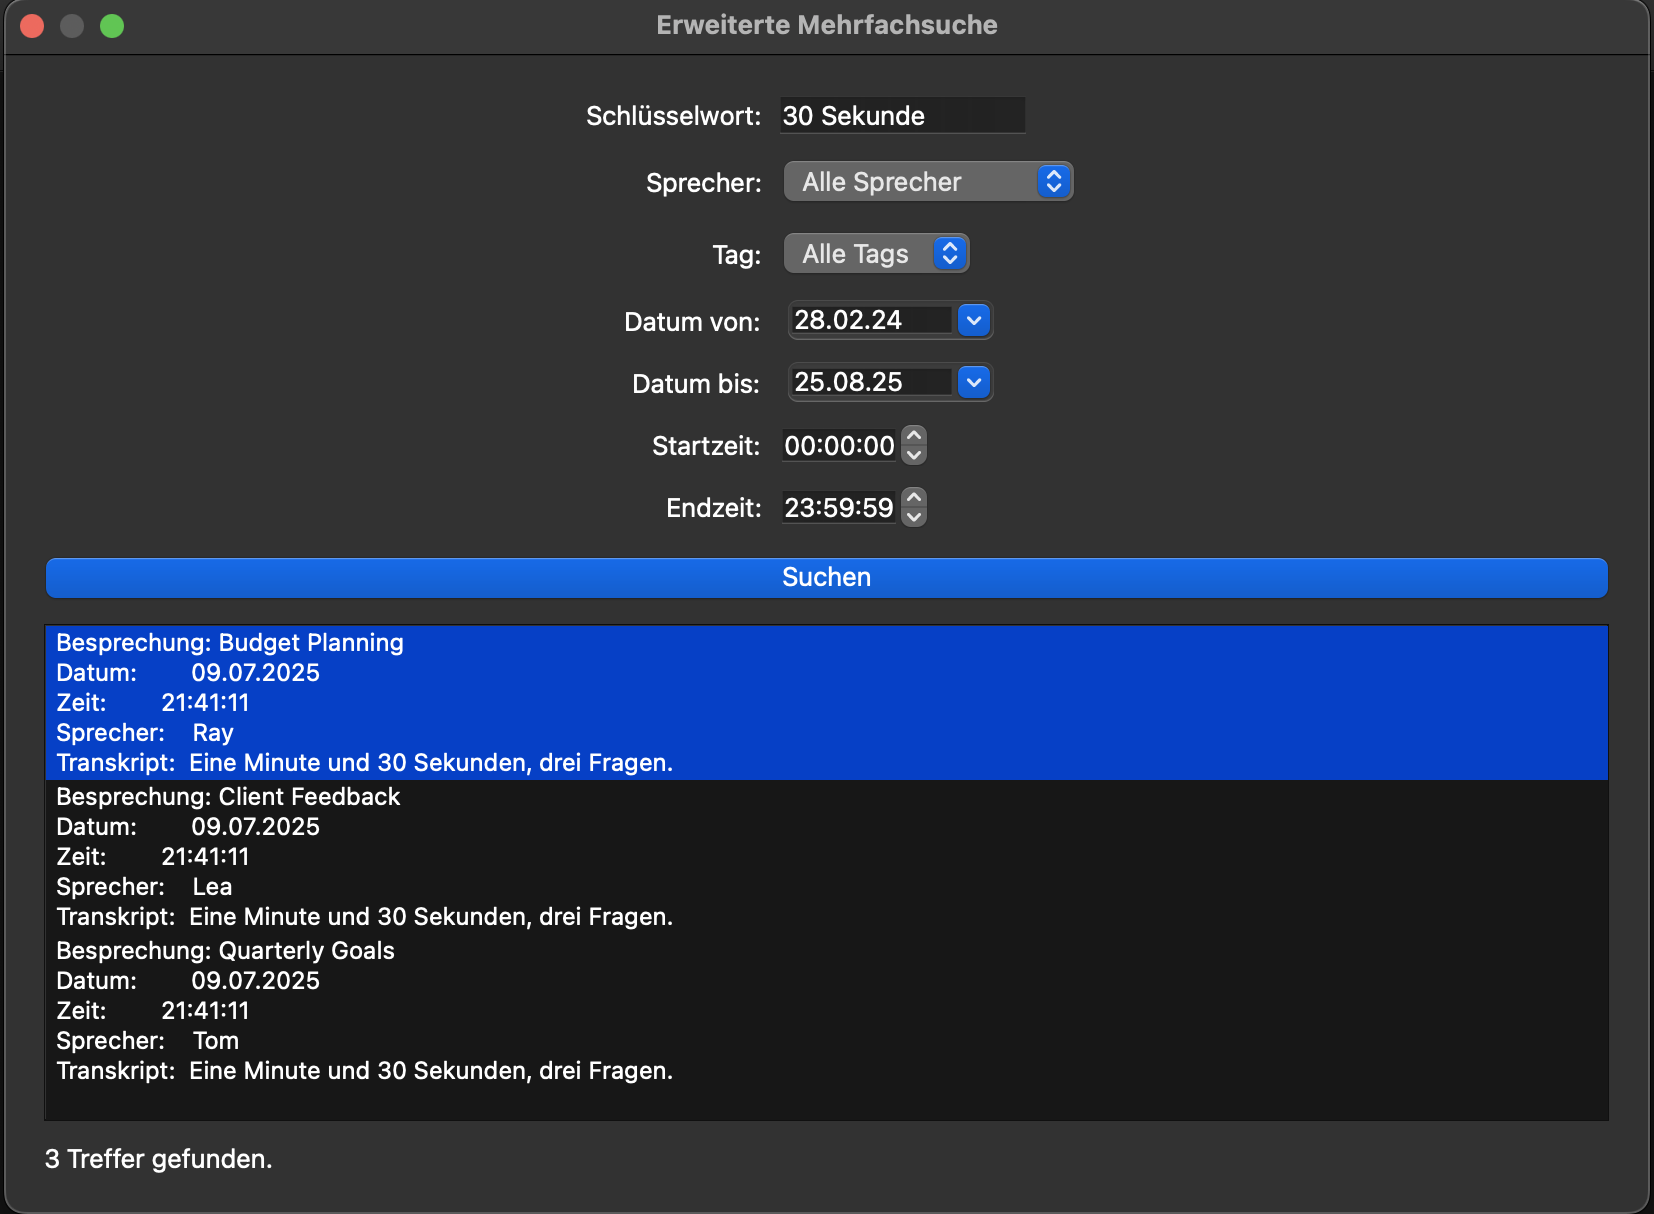
\includegraphics[width=0.7\linewidth]{Bilder/globaleSuche.png}
\caption[Protokolsuche]{Systemansicht: Suche über alle Transkripte}
\label{pic:globalesuche}
\end{figure}

Die Suchergebnisse werden in einer zentralen Liste angezeigt und enthalten neben dem Namen der Sitzung, dem Datum und dem Sprecher auch den Ausschnitt der Aussage, in dem das gesuchte Schlüsselwort vorkommt. Wie in Abbildung  \ref{pic:globalesuche}  dargestellt, kann durch Anklicken eines Eintrags direkt das entsprechende Meeting im Hauptfenster geladen werden. Dort werden die gesuchten Begriffe im Transkript hervorgehoben, sodass die relevanten Stellen unmittelbar erkennbar sind (Siehe Abbildung \ref{pic:markiertertreffer}). 

\begin{figure}[h]
\centering
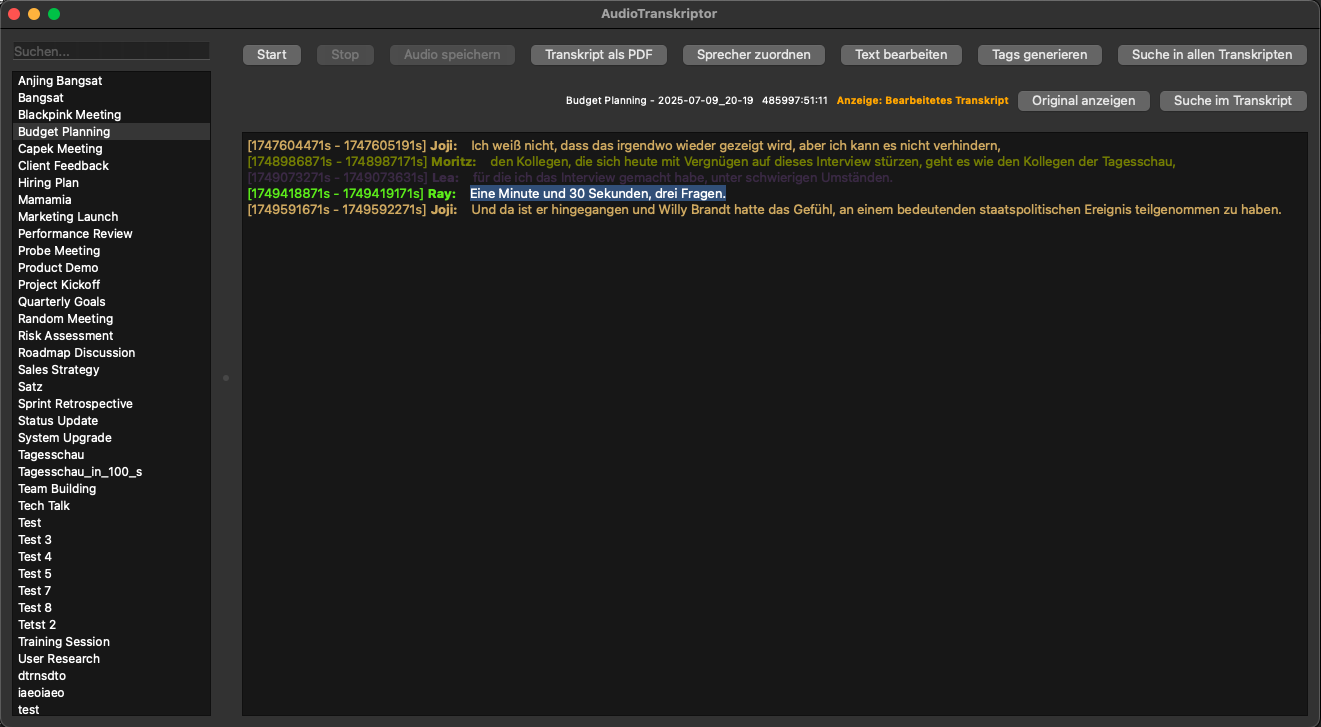
\includegraphics[width=0.7\linewidth]{Bilder/markierterTreffer}
\caption[Protokolsuche]{Darstellung eines Transkripts mit hervorgehobenen Suchergebnissen nach Auswahl eines Eintrags aus der Ergebnisliste}
\label{pic:markiertertreffer}
\end{figure}

\section{Workflow aus Anwendersicht}
\label{sec:workflow}
\authormargin{Mike Wild}

Angenommen man hat das Programm schon einmal gestartet, sodass die Python-Umgebung richtig aufgesetzt ist, dann sieht der typische Workflow mit dieser Applikation wie folgt aus. Das Programm startet mit dem Hauptfenster (vgl. Abschnitt \ref{sub:main}, Seite \pageref{sub:main}). Man drückt auf \glqq Start\grqq , hält sein Online-Meeting ab und drückt auf \glqq Stop\grqq . Danach kann man die Audiodatei speichern. Anschließend ordnet man den Sprecher die entsprechenden Namen zu, korrigiert ggf. den Text, generiert Schlagworte für das Transkript und speichert es in der Datenbank. Bei Bedarf exportiert man das Transkript als PDF-Datei. Danach ist man bereit für das nächste Meeting.

